\chapter{Scaling with reference size} \label{ch:trie}
\graphicspath{{\dir/}}

In this chapter we consider the problem of semi-global alignment of a set of
reads to a general graph reference. We supplement the reference graph with a
trie index and run shortest path algorithms (Dijkstra and \A with a very simple
heuristic) that start aligning from the trie root. We demonstrate that using a
trie index enables sublinear scaling of the alignment time with the reference
size. Even for moderate size references, we rearch orders of magnitude of
speedup compared to other optimal algorithms.

\section{Task Description: Alignment to Reference Graphs} \label{sec:task}

We now describe the task of aligning a query to a reference graph. To this end,
we (i)~introduce the task of optimal alignment on a \emph{reference graph},
(ii)~formalize this task in terms of an \emph{edit graph}, and (iii)~introduce an
alternative formulation in terms of an \emph{alignment graph}, which is the
basis for shortest path formulations of the optimal alignment.
%
\cref{fig:graph-constructions} summarizes these different graph types.

\para{Reference Graph}
We encode the collection of references to which we want to align in a reference
graph, which captures genomic variation that a linear reference cannot
express~\cite{paten_genome_2017,garrison_variation_2018}.
%
We formalize a reference graph as a tuple $\RG=(\RGV,\RGE)$ of nodes $\RGV$ and
directed, labeled edges $\RGE \subseteq \RGV \times \RGV \times \Sigma$, where
the alphabet $\Sigma=\{\texttt{A},\texttt{C},\texttt{G},\texttt{T}\}$ represents
the four different nucleotides.
%
Note that in contrast to sequence graphs~\cite{rautiainen_aligning_2017}, we
label edges instead of nodes.

\para{Path, Spelling}
Any path $\pi=(e_1,\dots,e_k) \text { in } \RG$ induces a \emph{spelling}
$\sigma(\pi) \in \Sigma^*$ defined by $\sigma(e_1)\cdots\sigma(e_k)$, where
$\sigma(e_i)$ is the label of edge $e_i$ and $\Sigma^* := \bigcup_{k \in
\mathbb{N}} \Sigma^k$. We note that our approach naturally handles cyclic walks
and does not require cycle unrolling, a feature shared with
\bitparallel~\cite{rautiainen_bitparallel_2019} and
\brownie~\cite{heydari_browniealigner_2018} but missing from
\vg~\cite{garrison_variation_2018}, \pasgal~\cite{jain_accelerating_2019} and
\valigntool~\cite{kavya_sequence_2019}.

\para{Alignment on Reference Graph}
An \emph{alignment} of \emph{query} $q \in \Sigma^*$ to a reference graph
$\RG=(\RGV,\RGE)$ consists of (i)~a path $\pi \text{ in } \RG$ and (ii)~a
sequence of edit operations (matches, substitutions, insertions, deletions)
transforming $\sigma(\pi)$ to~$q$.

\para{Optimal Alignment, Edit Distance}
Each edit operation is associated with a real-valued cost ($\cmatch$, $\csubst$,
$\cins$, and $\cdel$, respectively).
An optimal alignment minimizes the total cost of the edit operations converting
$\sigma(\pi)$ to $q$. For optimal alignments, this total cost is equal to the
edit distance between $\sigma(\pi)$ and $q$, i.e., the cheapest sequence of edit
operations transforming $\sigma(\pi)$ into $q$.

We make the (standard) assumption that $0 \leq \cmatch \leq \csubst, \cins,
\cdel$, which will be a prerequisite for the correctness of our approach.

\begin{figure}[t]
	\centering
	
\includegraphics[width=1\columnwidth]{./figs/edit_graph}
	\caption{Starting from the reference graph (left), we can construct the edit graph (middle) and the alignment graph $\AG$ for query $q=``\texttt{A}"$ (right). Edges are annotated with labels and/or costs, where sets of labels represent multiple edges, one for each letter in the set (indicated by $``\text{x}3"$ and $``\text{x}4"$).}
	\label{fig:graph-constructions}
\end{figure}

\paragraph{Edit Graph}
Instead of representing alignments as pairs of (i)~paths in the reference graph and
(ii)~sequences of edit operations on these paths, we introduce \textit{edit
graphs} whose paths intrinsically capture both. This way, we can
formally define an alignment more conveniently as a path in an edit graph.

Formally, an \emph{edit graph} $\AG:=(\AGV,\AGE)$ has directed, labeled edges
$\AGE \subseteq \AGV \times \AGV \times \Sigma_\epsilon \times \mathbb{R}_{\geq
0}$ with associated costs that account for edits. Here, $\Sigma_\epsilon :=
\Sigma \cup \{\epsilon\}$ extends the alphabet $\Sigma$ by $\epsilon$ to account
for deleted characters (see \cref{fig:graph-constructions}).
%
The edit and reference graphs consist
of the same nodes, i.e., $\AGV=\RGV$. However, $\AGE$ contains more edges
than $\RGE$ to account for edits.
%
Concretely, for each edge $(u,v,\ell) \in \RGE$, $\AGE$ contains edges to
account for (i)~matches, by an edge $(u,v,\ell,\cmatch)$, (ii)~substitutions, by
edges $(u,v,\ell',\csubst)$ for each $\ell' \in \Sigma \backslash \ell$,
(iii)~deletions, by an edge $(u,v,\epsilon,\cdel)$, and (iv)~insertions, by
edges $(u,u,\ell',\cins)$ for each $\ell' \in \Sigma$.
%
The spelling $\sigma(\pi) \in \Sigma^*$ of a path $\pi \in \AG$ is defined
analogously to reference graphs, except that deleted letters (represented by
$\epsilon$) are ignored. The cost $\cost{\pi}$ of a path $\pi \in \AG$ is the
sum of all its edge costs.

\paragraph{Alignment on Edit Graph}
An \emph{alignment} of query $q$ to $\RG$ is a path $\pi \text{ in } \AG$
spelling $q$, i.e., $q=\sigma(\pi)$. An \emph{optimal alignment} is an alignment
of minimal cost.


\para{Alignment Graph}
To find an optimal alignment of $q$ to the edit graph $\EG$ using shortest path
finding algorithms, we must ensure that only paths spelling $q$ are considered.
To this end, we introduce an alternative but equivalent formulation of
alignments in terms of an \emph{alignment graph} $\AG=(\AGV,\AGE)$.

Here, each \emph{state} $\langle v,i \rangle \in \AGV$ consists of a vertex $v \in
\EGV$ and a query position $i \in \{0,\dots,|q|\}$ (equivalent
to~\cite{rautiainen_aligning_2017}). Traversing a state $\langle v,i \rangle \in
\AGV$ represents the alignment of the first $i$ query characters ending at node $v$.
%
In particular, query position $i=0$ indicates that we have not yet matched any
letters from the query.
%
We note that the alignment graph explicitly depends on the query $q$. In
particular, the example alignment graph $\AG[``\texttt{A}"]$ in
~\cref{fig:graph-constructions} lacks substitution edges from $\EG$, as their
labels ($\texttt{C}$, $\texttt{G}$, $\texttt{T}$) do not match the query
$q=``A"$.

We construct the alignment graph $\AG$ to guarantee that any walk from a source
$\langle u,0 \rangle$ to a state $\langle v,i \rangle$ corresponds to an
alignment of the first $i$ letters of query $q$ to $\RG$. As a consequence,
there is a one-to-one correspondence between alignments $\edit{\pi}$ of $q$ to
$\EG$ and paths $\alignment{\pi} \in \AG$ from sources $S:=\RGV \times \{0\}$ to
targets $T:=\RGV \times \{|q|\}$, with
$\cost{\reference{\pi}}=\cost{\alignment{\pi}}$. To find the best alignment in
$\EG$, only paths in $\AG$ (walks without repeating nodes) can be considered,
since repeating a node in $\AG$ cannot lead to a lower cost ($\cdel \geq 0$) for
the same state.

\begin{samepage}
The edges $\AGE \subseteq \AGV \times \AGV \times \Sigma_\epsilon \times
\mathbb{R}_{\geq 0}$ are built based on the edges in $\EGE$, except that the
former (i)~keep track of the position in the query $i$, and (ii)~only contain
empty edges or edges
whose label matches the next query letter:

\vspace{-0.7em}
{%
\small
\begin{alignat}{10}
	(u,v,\ell,w) &\in \EGE \implies (&\langle u, i \rangle, &\langle v, i+1
		&&\rangle,\ell,w) \in \AGE \quad \text{ for } 0 \leq i < |q| \text{ with }
		q[i]=\ell \label{eq:alignment-edges-nondeletions} \\
	(u,v,\epsilon,w) &\in\EGE \implies (&\langle u, i \rangle, &\langle v, i
		&&\rangle,\epsilon,w) \in \AGE \quad \text{ for } 0 \leq i < |q| \label{eq:alignment-edges-deletions}
\end{alignat}
}%
\end{samepage}
%
Here, assuming $0$-indexing, $q[i]$ is the next letter to be matched after
matching $i$ letters. Then, \cref{eq:alignment-edges-nondeletions} represents
matches, substitutions, and insertions (which advance the position in the query
by $1$), while \cref{eq:alignment-edges-deletions} represents deletions (which do
not advance the position in the query).

\para{Dynamic Construction}
As the size of the alignment graph is $\Oh(\lvert \RG \rvert \concat \lvert q
\rvert)$, it is expensive to build it fully for every new query.
Therefore, our implementation constructs the alignment graph $\AG$ on-the-fly:
the outgoing edges of a node are only generated on demand and are freed from
memory after alignment.

\section{Overview}

We present an algorithm for the \emph{optimal alignment} of sequences to
\emph{genome graphs}. It works by phrasing the edit distance minimization task
as finding a shortest path on an implicit alignment graph. To find a shortest
path, we instantiate the \A paradigm with a novel domain-specific heuristic
function that accounts for the upcoming subsequence in the query to be aligned,
resulting in a provably optimal alignment algorithm called \astarix.
Experimental evaluation of \astarix shows that it is 1--2 orders of magnitude
faster than state-of-the-art optimal algorithms on the task of aligning Illumina
reads to reference genome graphs.

All optimal algorithms have to iterate over the whole reference for each query.
We should be able to optimize this by precomputation.

\paragraph{Methods}
We introduce a novel approach, called \astarix, for optimal sequence-to-graph
alignment based on \A. As with any \A instantiation, the core difficulty lies in
developing an accurate domain-specific heuristic which is fast to compute. We
design a heuristic that accounts for the content of the upcoming query letters
to be aligned, which more effectively guides the search. Our proposed heuristic
has two advantages: (i)~it is correctness-preserving, that is, it preserves the
fact that \astarix finds the best alignment, yet (ii)~it is practically
effective in that the algorithm performs a near-optimal number of steps.
Overall, this heuristic enables \astarix to compute the best alignment while
also scaling to larger reference graph sizes when compared to existing
state-of-the-art optimal aligners.

\paragraph{Results}
% From outside
%In the context of semi-global sequence-to-graph alignment, \A has been used to
%empirically scale sublinearly with the reference size for short reads.

\begin{samepage}
The main contributions presented in this chapter are:
	
\begin{enumerate}
	\item \textbf{\astarix.} An algorithm for optimal sequence-to-graph
	alignment based on a novel instantiation of \A with an accurate
	domain-specific heuristic that accounts for the upcoming query letters to be
	aligned (\cref{TRIEsec:astarix-algo}).
	\item \textbf{Algorithmic optimizations.}
	To ensure that \astarix is practical, we introduce a number of algorithmic
	optimizations which increase performance and decrease memory footprint
	(\cref{TRIEsec:optimizations}). We also prove that all optimizations are
	correctness-preserving.
	\item \textbf{Thorough experimental evaluation of \astarix.}
	We demonstrate that \astarix is up to 2 orders of magnitude faster than
	other optimal aligners on various reference graphs (\cref{TRIEsec:eval}).
\end{enumerate}
\end{samepage}

\section{\astarix: Finding Optimal Alignments Using \A} \label{sec:astarix-algo}
In this section, we first introduce the general \A algorithm for finding
shortest paths, and the notion of an optimistic heuristic, a sufficient
condition for instantiations of \A to be correct (i.e., to indeed find shortest
paths). Then we instantiate \A with our domain-specific heuristic that accounts
for upcoming subsequences to be aligned, and prove that this heuristic is
optimistic.

\begin{algorithm}[t]
	\caption{\astarix including heuristic function.}\label{TRIEalg:astarix}
	\begin{algorithmic}[1]
		\State $\RG$: Reference graph \label{TRIElin:reference}
		\Comment Global variables
		\State $d$: Upcoming sequence length \label{TRIElin:d}
		\Statex
		\Function{AStarix}{$q\colon \text{Query}$} \label{TRIElin:astarix}
			\State $\AG \gets \Call{DefineAlignmentGraph}{\RG, q}$
			\Comment Following \cref{TRIEsec:task}
			\State $S \gets \{\langle v,i \rangle \in \AGV \mid i=0 \}$ \label{TRIElin:starts}
			\Comment Sources: no letter matched
			\State $T \gets \{\langle v,i \rangle \in \AGV \mid i=|q| \}$
			\Comment Targets: all letters matched
			\State \Return $\Call{\A}{\AG, S, T, \textsc{Heuristic}}$
			\Comment \A provided in \cref{TRIEapp:astar} \label{TRIElin:ret}
		\EndFunction
		\Statex
		\Function{Heuristic}{$\langle u, i \rangle\colon \text{State}$} \label{TRIElin:heuristic-start}
		\Comment Heuristic: Cost of upcoming sequence
			\State $d' \gets \min(d, |q|-i)$
			\Comment Actual length of upcoming sequence
			\State $s \gets q[i:i+d']$ \label{TRIElin:s}
			\Comment Upcoming sequence (next $d$ letters after current)
			\State \Return $\Call{$h$}{u, s}$
			\label{TRIElin:align-upcoming}
			\Comment Cost of aligning $s$ to $\RG$ starting from $u$
		\EndFunction \label{TRIElin:heuristic-end}
		\Statex
		\Function{$h$}{$u, s$}
		\Comment Cost of aligning $s$ starting from $u$
			\State \Return $\Call{RecursiveAlign}{u, s, 0.0, \infty}$
			\Comment Simple branch-and-bound \label{TRIElin:recursive-align}
		\EndFunction
	\end{algorithmic}
\end{algorithm}

\subsection{Background: General \A algorithm} \label{subsec:general-astar}
Given a weighted graph $G=(V,E)$ with $E \subseteq V \times V \times
\mathbb{R}_{\geq 0}$, the \A algorithm (abbreviated as \A) searches for the
shortest path from sources $S \subseteq V$ to targets $T \subseteq V$. It is an
extension of Dijkstra's algorithm that additionally leverages a \emph{heuristic
function} $h \colon V \to \mathbb{R}_{\geq 0}$ to decide which paths to explore
first.
%
If $h(u) \equiv 0$, \A is equivalent to Dijkstra's algorithm.
%
We provide an implementation of \A and Dijkstra in \cref{app:astar}, but do not
assume knowledge of either algorithm in the following.
%
At a high level, \A maintains the set of all \emph{explored} states, initialized
with the set of sources $S$. Then, \A iteratively \emph{expands} the explored
state with lowest estimated cost by exploring all its neighbors, until it finds
a target. Here, the cost for node $u$ is estimated by the distance from source, called $g(u)$, plus the estimate from the heuristic $h(u)$.


\para{Heuristic Function}
The heuristic function $h(u)$ estimates the
cost $h^*(u)$ of a shortest path in $G$ from $u$ to a target $t \in T$. Intuitively, a
good heuristic correlates well with the distance from $u$ to $t$.

To ensure that \A indeed finds the shortest path, $h$ should be
\emph{optimistic}:

\begin{definition}[Optimistic heuristic] A heuristic $h$ is \textit{optimistic}
    if it provides a lower bound on the distance to the closest target: $\forall u. h(u) \leq h^*(u)$.
\end{definition}

While any optimistic $h$ ensures that \A finds optimal
alignments~\cite[Res.~3]{dechter_generalized_1985}, the specific choice of $h$
is critical for performance. In particular, decreasing the error $\delta(u) =
h^*(u)-h(u)$ can only improve the performance of
\A~\cite[Res.~6]{dechter_generalized_1985}. Thus, a key contribution of ours is a domain-specific heuristic $h$.


\subsection{\astarix: Instantiating \A} \label{subsec:astarix-heuristic}
\cref{alg:astarix} shows an unoptimized version of \astarix and its heuristic
function.
%
\astarix expects a reference graph (\cref{lin:reference}) and a query
(\cref{lin:astarix}) as input, and returns an optimal alignment (\cref{lin:ret})
by searching for a shortest path from $S$ to $T$ in the alignment graph $\AG$.
It is parameterized by hyper-parameters ($d$ in \cref{lin:d}, more in
\cref{sec:optimizations}) and edit costs (implicitly provided).

The function \textsc{Heuristic}
(\crefrange{lin:heuristic-start}{lin:heuristic-end}) computes a lower bound on
the remaining cost of a best alignment: the minimum cost $h(u,s)$ of aligning
the \emph{upcoming sequence} $s$ (where $\lvert s \rvert \leq d$) starting from
node $u$. Importantly, $s$ is limited to the next $d' \leq d$ letters of $q$,
starting from query position $i$. Thus, computing $h(u,s)$ is substantially
cheaper than aligning all remaining letters of $q$.

To compute $h(u,s)$ we leverage a simple branch-and-bound algorithm, provided in
\cref{app:recursive-align}. In the following, for convenience, we refer to the
heuristic as $h$ (which is parameterized by $(u,s)$) instead of
\textsc{Heuristic} (which is parameterized by $\langle u, i \rangle$). Further,
we say that $h$ is optimistic if $h(u,s)$ is a lower bound on the cost for
aligning all remaining letters (i.e., $q[i:|q|]$) starting from node $u$ (note
that $s$ is a prefix of $q[i:|q|]$).

\begin{samepage}
\begin{theorem} \label{thm:optimistic}
	$h$ is optimistic.
\end{theorem}
\begin{proof}
$h$ only considers the next $d'$ letters of $q$ instead of all
remaining letters. Since all costs are non-negative, the theorem follows.
\end{proof}
\end{samepage}

\begin{figure}[t]
	\centering
	
\includegraphics[width=0.9\columnwidth]{./figs/heuristic}
	\caption{The benefit of using our heuristic over \dijkstra. Alignment graph
	$\AG[``\texttt{ATAA}"]$ (right) is based on reference graph $\RG$ (left),
	but omits insertion and deletion edges for simplicity. The pink boxes $g+h$
	indicate the distance from the sources $S=\{\langle u,0 \rangle, \langle v,0
	\rangle \}$ (in $g$) and the cost of aligning the next $d=2$ letters (in
	$h$). \dijkstra (resp. \A) expands states circled in
	\textcolor{my-full-blue}{blue} (resp.
	\textcolor{my-full-red}{dashed red}).}
	\label{fig:heuristic-benefit}
\end{figure}

\para{Benefit of \A Heuristic over \dijkstra} \label{para:heuristic-benefits}
\cref{fig:heuristic-benefit} shows the benefit of using our heuristic function
compared to \dijkstra. Here, \dijkstra expands states based on their distance
$g$ from the origin nodes $\st{u}{0}$ and $\st{v}{0}$. Hence, depending on
tie-breaking, \dijkstra may expand all states with $h \leq 1$, as shown in
\cref{fig:heuristic-benefit}. By contrast, \A chooses the next state to expand
by the sum of the distance from the origin $g$ and the heuristic $h$, expanding
only states with $g+h \leq 1$.

\para{Memoization} \label{para:memoization}
Recall that the return value of $h$ in \cref{lin:heuristic-start} only depends
on $u$ and the upcoming sequence $s$ (which in turn depends on $i$ and $d$).
Thus, $h(u,s)$ can be reused for different positions across different queries in
$\Oh(1)$ time, if it was computed for a previous query.
\section{\astarix Algorithm: Optimizations} \label{sec:optimizations}
We now discuss several optimizations we developed to speed up \astarix while
preserving its optimality. These optimizations reduce preprocessing and
alignment runtime as well as memory footprint (in particular for memoization).

\subsection{Reducing Semi-global to Local Alignment Using a Trie} \label{TRIEsubsec:trie}
To find an optimal alignment, we generally need to consider all reference graph
nodes $u \in \RG$ as possible starting nodes. Thus, optimal aligners
\pasgal~\cite{jain_accelerating_2019} and
\bitparallel~\cite{rautiainen_bitparallel_2019} brute-force through all
possible starting nodes $u \in \RG$.

To more efficiently handle arbitrary starting positions for alignments, we
extend the reference graph with a trie (referred to as \textit{suffix tree}
in~\cite{dox2018efficient}) to effectively align from all possible starting
nodes \emph{simultaneously}.

\para{Single Starting State}
In the trie approach, abstraction nodes are added to the graph, each of which
corresponds to a set of nodes in $\RG$ that correspond to the same prefix. In
the following, we formalize this approach.

Concretely, we extend $\RG$ by a \emph{trie of depth $D$}, resulting in graph
$\TG=(\TGV,\TGE)$. Our goal is that all paths in $\RG$ that have length $D$ and
end in $v \in \RGV$ correspond to paths in $\TG$ starting from a single source
$\epsilon$ to $v \in \TGV$, where $\epsilon$ represents the empty string. This
correspondence ensures that it suffices to consider only paths in $\TG$ starting
from the source $\epsilon$. In particular, each alignment on $\TG$ can
be translated into an alignment on $\RG$ (we omit this translation
here).

\begin{wrapfigure}{r}{0.48\linewidth}
	%\vspace{-20pt}
	\centering
	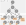
\includegraphics[width=\linewidth]{figs/tree}
	\caption{$\TG$ enables semi-global alignment by extending $\RG$ with a trie.}
	\label{TRIEfig:trie}
	\vspace{-25pt}
\end{wrapfigure}
\cref{TRIEfig:trie} shows an example trie. To construct it, we first associate with
every node $v \in \RGV$ the set $\mathcal{S}_v$ of its $D$-mers (orange boxes in
\cref{TRIEfig:trie}): spells of paths ending in $v$ and of length $D$. Our goal is
then to use paths in the trie to spell these $D$-mers.

Second, we construct the trie nodes from all prefixes of these $D$-mers:
%
$$ \TGV:= \RGV \cup
\bigcup_{v \in \RGV} \left\{s[0:i] \,\middle|\, \begin{array}{c}
	s \in \mathcal{S}_v, \\
	0 \leq i < D
\end{array} \right\}.
$$

Third, we add edges within the trie, which ensure that paths from $\epsilon$ to
any trie node $s$ spell $s$. Formally, whenever $s \concat \ell \in \TGV$, we add
an edge $(s,s \concat \ell, \ell)$ to $\TGE$, where ``$\concat$'' denotes string
concatenation.
%
Finally, we add edges between the trie and the reference graph, which ensure
that any $D$-mer of any node $v \in \RGV$ can be spelled by a walk from
$\epsilon$ to $v$. Formally, if $s \concat \ell \in \mathcal{S}_v$, then
$(s,v,\ell) \in \TGE$.

Importantly, extending $\RG$ to $\TG$ is compatible with the construction of the
edit graph $\EG$, the construction of the alignment graph and all other
optimizations. In particular, when searching for a shortest path in the
alignment graph constructed from $\TG$, it suffices to only consider starting
node $\langle \epsilon, 0 \rangle$.

\para{Reducing Size of Trie} \label{TRIEpara:reducing_trie}
We can reduce the size of the trie by removing specific trie nodes.
%
In particular, we iteratively remove each trie leaf node $s \cdot \ell \in \TGV$ with a unique outgoing edge $(s \cdot \ell, v, \ell')$ to a reference graph node $v \in \RGV$.
%
To compensate for removing node $s \cdot \ell$, we introduce a new edge $(s, u, \ell)$ to a node $u \in \RGV$ with an edge $(u,v,\ell')$ (such a node must exist according to the construction of $\TG$).
%
For example, in \cref{TRIEfig:trie}, we (i)~remove node \texttt{AT} including its edges $(\texttt{A},\texttt{AT},\texttt{T})$ and $(\texttt{AT},u_3,\texttt{C})$, but (ii)~introduce an edge $(\texttt{A},u_2,T)$.

This optimization is lossless, as the $D$-mer $s \cdot \ell \cdot \ell' \in \mathcal{S}_v$ can still be spelled by the path from $\epsilon$ to $s$, extended by $(s, u, \ell)$ and $(u, v, \ell')$.

\subsection{Greedy Match Optimization} \label{subsec:greedy}
We also employ an optimization originally developed for computing the edit
distance between two strings~\cite{sellers_algorithm_1974,allison_lazy_1992}, but
which has also been used in the context of string to graph
alignment~\cite{dox2018efficient}. We omit the correctness proof of this
optimization, which is already covered
in~\cite{sellers_algorithm_1974}, and only explain the intuition behind it.

Suppose there is only one outgoing edge $e = (u, v, \ell) \in \RGE$ from a node
$u \in \RGV$. Suppose also that while aligning a query $q$, we explore state
$\st{u}{i}$ for which the next query letter $q[i]$ matches the label $\ell$. In
this case, we do not need to consider the edit outgoing edges, because
any edit at this point can be postponed without additional cost, as $\cmatch
\leq \min(\csubst, \cins, \cdel)$. Thus, we can greedily explore state
$\st{v}{i+1}$, aligning $q[i+1]$ to $e$ by using the edge $(\st{u}{i},
\st{v}{i+1}, \ell, \cmatch)$ before continuing with the \A search.
We note that this optimization is only applicable when aligning in non-branching
regions of the reference graph. In particular, it is not applicable for most
trie nodes (\cref{subsec:trie}).

\subsection{Speeding Up Evaluation of Heuristic} \label{subsec:speedup-heuristic}
In the following, we show how to reduce the runtime of evaluating the heuristic
$h(u,s)$, by introducing two separate optimizations that compose naturally.

\para{Capping Cost} We cap $h(u,s)$ at $\costcap$, replacing it by
$h_{\costcap}(u,s):=\min(h(u,s),\costcap)$. To achieve this, we allow
\textsc{RecursiveAlign} to ignore paths costing more than $\costcap$.
%
For large enough $\costcap$, this speeds up computation without significantly
decreasing the benefit of the heuristic, since nodes associated with a high
heuristic value are typically not explored anyways. We investigate the effect of
$\costcap$ in \cref{subsec:parameter_estimation}.

\begin{samepage}
	\begin{thm} \label{thm:hbar_optimistic}
		$h_{\costcap}$ is optimistic.
	\end{thm}
	\begin{proof}
		We have $h_\costcap(u,s) \leq h(u,s)$ and that $h(u,s)$ is
		optimistic (\cref{thm:optimistic}).
	\end{proof}
	\end{samepage}

\para{Capping Depth}
We reduce the number of nodes that need to be considered by $h(u,s)$. To this
end, we define a modified heuristic $h_d(u,s)$ that only considers nodes $R_u
\subseteq \EGV$ at distance at most $d$ from $u$ (cp. \cref{lin:d} in
\cref{alg:astarix}):
$
R_u := \{ v \in \RGV \mid \exists \; \text{path } \pi \in \EG \text{ from } u \text{ to } v \text{ with } \lvert \pi \rvert \leq d \}
$.

If an alignment of $s$ reaches the boundary of $R_u$, defined as $$B(R_u) := \{v
\in R_u \mid \exists (v,v',\ell) \in \EGE \text{ with } v' \notin R_u \},$$ it is
allowed to only spell a prefix of $s$, and the remaining unaligned letters of
$s$ are considered aligned with zero cost:
\begin{gather*}
h_d(u,s) := \min_{\pi \in \Pi} \cost{\pi}, \text{ where } \\
\Pi := \left\{ \pi \in \RG \;\middle|\; \begin{array}{c}
\mli{start}(\pi)=u, 
\sigma(\pi)=s \lor \big(\mli{end}(\pi)\in B(R_u) \land \exists i. \sigma(\pi)=s[1..i] \big)
\end{array}
\right\}
\end{gather*}

\begin{samepage}
\begin{thm} \label{thm:hbar_optimistic}
	$h_d$ is optimistic.
\end{thm}
\begin{proof}
It suffices to show $h_d(u,s) \leq h(u, s)$ since $h(u, s)$ is optimistic. In
the case where all of $s$ is aligned, $h_d(u,s) = h(u, s)$. Otherwise, the
unaligned letters of $s$ are not penalized, so $h_d(u,s) \leq h(u, s)$.
\end{proof}
\end{samepage}


\subsection{Partitioning Nodes into Equivalence Classes} \label{subsec:partition}
We have shown in \cref{para:memoization} how to reuse an already computed
$h(u,s)$ for repeating $s$ across different queries and query positions. In the
following, we additionally aim to reuse $h(u,s)$ across different nodes $u$, so
that $h(u,s)$ does not need to be computed for all nodes $u$. Intuitively, we
want to assign two nodes $u$ and $v$ to the same equivalence class when the
\emph{graph region} considered by $h(u,s)$ is equivalent to the graph region
considered by $h(v,s)$, up to renaming of nodes.

Thus, $h(u,s)=h(v,s)$ if $u$ and $v$ are from the same equivalence class.
Therefore, we can (arbitrarily) choose a representative node $r \in \RGV$ for
every equivalence class, and evaluate $h(r,s)$ instead of $h(u,s)$, where $r$ is
the representative of the equivalence class of $u$. To look up representative
nodes in $\Oh(1)$, we define a helper array $\mli{repr}$ with $\mli{repr[u]} =
r$.

\para{Identifying Equivalence Classes}
To identify the nodes belonging to the same equivalence class, we assume the
optimization from \cref{subsec:speedup-heuristic}, \ie, that our heuristic only
considers nodes up to a distance $d$ from~$u$.
%
Moreover, for performance reasons, our implementation detects only the
equivalence classes of nodes $u$ with a single outgoing path of length at least
$d$.
%
In this case, $u$ and $u'$ are in the same equivalence class if their outgoing
paths spell the same sequence.
%
In contrast, we leave nodes with forking paths in separate equivalence classes.

Note that for smaller $d$, the number of equivalence classes gets smaller, the
reuse of the heuristic gets higher, and the memoization table has a lower memory
footprint. At the same time, however, the heuristic $h_d(u,s)$ is less
informative.

\section{Results} \label{sec:evals}

Our algorithm is implemented in the aligner
\astarpa%
\footnote{\url{https://github.com/RagnarGrootKoerkamp/astar-pairwise-aligner/tree/1e3841}}
in Rust. We compare it with state of the art exact aligners on
synthetic~(\cref{GLOBALsec:evals-comparison-synthetic}) and
human~(\cref{GLOBALsec:evals-comparison-hg})
data%
\footnote{\url{https://github.com/pairwise-alignment/pa-bench/releases/tag/datasets}}
using \pabench%
\footnote{\url{https://github.com/pairwise-alignment/pa-bench/commit/55db710}}%
.
We justify our heuristics and optimizations by comparing their scaling and
performance~(\cref{sec:techniques}).

\begin{figure*}[t]
    %\vspace{-1.66em}
    \centering
    \hfill
    \subfloat[Runtime scaling with length ($d{=}4\%$, $r{=}1$)]
    {\includegraphics[scale=0.55]{plots/scaling_n.labels.pdf}\label{fig:scaling-n}}
    \hfill
    \subfloat[Runtime scaling with length ($d{=}12\%$, $r{=}2$)\!\!]
    {\includegraphics[scale=0.55]{plots/tools_e0.15_enlarged.labels.pdf}\label{fig:scaling-n-large}}
    \hfill
    \subfloat[Runtime scaling with divergence]
    {\includegraphics[scale=0.55]{plots/scaling_e.labels.pdf}\label{fig:scaling-e}}
    \hfill
    \caption[Runtime scaling on synthetic data]{
      \textbf{Runtime comparison on synthetic data}
      \protect\subref{fig:scaling-n}\protect\subref{fig:scaling-n-large}
  Log-log plots comparing our simplest~(\SH) and most accurate
  heuristic~(\GCH with DT) to \edlib, \wfa, and other algorithms
      (averaged over $10^6$ to $10^7$ total bp, seed length $k{=}15$).
  The slopes of the bottom (top) of the dark-grey cones correspond to linear (quadratic) growth.
      \SH without
      pruning is dotted, and variants with DT are solid. At $4\%$ divergence,
      the complex techniques \CSH, \GCH, and DT (not shown) are as fast as \SH.
  Missing data points are due to exceeding the $\qty{32}{GiB}$ memory limit.
  \protect\subref{fig:scaling-e}
  Runtime scaling with divergence ($n{=}10^4$, $10^6$ total bp, $k{=}10$).
      \GCH (not shown) is as fast as \CSH.}
    \label{fig:synthetic}
\end{figure*}

\subsection{Setting} \label{GLOBALsec:evals-setup}

\paragraph{Synthetic data}
We measure the performance of aligners on a set of randomly-generated sequences.
Each set is parametrized by the number of sequence pairs, the sequence length
$n$, and the error rate $e$. The first sequence in a pair is generated by
concatenating $n$ i.i.d. letters from $\Sigma$. The second sequence is generated
by sequentially applying $\lfloor e{\cdot} n\rfloor$ edit operations (insertions,
deletions, and substitutions with equal probability) to the first sequence. Note
that errors can cancel each other, so the final distance between the sequences
is usually less than $\lfloor e{\cdot} n \rfloor$. In order to minimize the
measurement errors, each test consists of a number of sequence pairs.

\paragraph{Human data}
We consider two datasets%
\footnote{\url{https://github.com/RagnarGrootKoerkamp/astar-pairwise-aligner/releases/tag/datasets}}
of Oxford Nanopore Technologies (ONT) reads that are aligned to regions of the
telomere-to-telomere assembly of a human genome
CHM13~(v1.1)~\citep{nurk2022complete}. Statistics are shown in~\cref{GLOBALtab:hg}.

\begin{itemize}
  \item \emph{CHM13: Human reads without biological variation.} We randomly
        sampled $50$ reads of length at least $500\kbp$ from the first
        $\qty{12}{GB}$ of the ultra-Long ONT reads that were used to assemble
        CHM13. We removed soft clipped regions and paired each read to its
        corresponding reference region in CHM13\footnote{\url{https://github.com/RagnarGrootKoerkamp/bam2seq}}.
  \item \emph{NA12878: Human reads with biological variation.} We consider the
        long ONT MinION reads from a different reference sample
        NA12878~\citep{bowden2019sequencing} which was used to evaluate
        \wfa~\citep{marco2022optimal}. This dataset contains $48$ reads longer than
        $500\kbp$ that were aligned to CHM13.
\end{itemize}

\begin{table}[t]
	\ra{0.8}
  \centering
  \sffamily
  \setlength{\tabcolsep}{3pt}
  \begin{tabular}{
    l
    c
    S[table-format=3]
    S[table-format=3]
    S[table-format=3]
    l
    S[table-format=1.1]
    S[table-format=1.1]
    S[table-format=2.1]
    }
    & \multirow{2.7}{4.8em}{\centering\textbf{Biological\newline
                       variation}} & \multicolumn{3}{c}{\textbf{Length} [\kbp]}
    &  & \multicolumn{3}{c}{\textbf{Error rate} [$\%$]} \\
    \cmidrule{3-5} \cmidrule{7-9}
    \textbf{Dataset} &&  {min} & {mean} & {max}  && {min} & {mean} & {max} \\
    \cmidrule{1-9}
    \datasetOne & No & 500 & 590 & 840 & & 2.7 & 6.3 & 18.0 \\
    \datasetTwo & Yes & 502 & 624 & 1053 & & 4.4 & 7.4 & 19.8 \\
    \cmidrule{1-9}
  \end{tabular}
  \caption[Statistics on the real data]{Statistics on the \textbf{real data}:
  ONT reads from human samples.}
  \label{GLOBALtab:hg}
\end{table}

\paragraph{Compared algorithms and aligners}
We compare the \sh and \csh, implemented in \astarpa, to the state-of-the-art exact
pairwise aligners \wfa and \edlib. In order to study the performance of the \A
heuristic functions and the pruning optimization, we also compare to \dijkstra's
algorithm (which is equivalent to \A with a zero heuristic) and to a no-pruning
variant of \A, all implemented in \astarpa. The exact aligners \seqan and
\parasail are not included in this evaluation since they have been outperformed
by \wfa and \edlib~\citep{marco2021fast}. We execute all aligners with unit edit
costs and compute not only the edit distance but also an optimal alignment.
See~\cref{GLOBALsec:app-tools} for aligner versions and parameters.

\paragraph{Execution}
All evaluations are executed on Arch Linux on a single thread on an
\texttt{Intel Core i7-10750H \mbox{CPU @ 2.6GHz}} processor with $\qty{64}{GB}$
of memory and $6$ cores, with hyper-threading and performance mode disabled. We fix
the CPU frequency to \texttt{2.6GHz} and limit the available memory per
execution to $\qty{30}{GB}$ using \texttt{ulimit -v 30000000}. To speed up the
evaluations, we run $3$ jobs in parallel, pinned to cores $0$, $2$, and $4$.

\paragraph{Measurements}
The runtime (wall-clock time) and memory usage (resident set size) of each run
are measured using \texttt{time}. The runtime in all plots and tables refers to
the average alignment time per pair of sequences. To reduce startup overhead,
we average faster alignments over more pairs of sequences, as specified in the figure
captions. Memory usage is measured as the maximum used memory during the
processing of the whole input file. To estimate how algorithms scale with
sequence length, we calculate best fit polynomials via a linear fit in the
log-log domain using the least squares method.

\paragraph{Parameters for the \A heuristics}
Longer sequences contain more potential locations for off-path seed matches
(\ie lying outside of the resulting optimal alignment). Each match takes time
to be located and stored, while also potentially worsening the heuristic. To
keep the number of matches low, longer seeds are to be preferred. On the other
hand, to handle higher error rates, a higher number of shorter reads is
preferable. For simplicity, we fix $k{=}15$ throughout our evaluations as a
reasonable trade-off between scaling to large $n$ and scaling to high $e$. We
use exact matches ($r{=}1$) for low error rates ($e {\leq} 5\%$), and inexact
matches ($r{=}2$) for high error rates ($e{\geq}10\%$). For human
datasets we use $r{=}2$ since they include sequences with error rates
higher than $10\%$.

\begin{figure}[H]
  \centering
  \includegraphics[scale=0.50]{plots/real_summary.pdf}
  \caption[Runtime of \astarpa on long human reads]{\textbf{Runtime on long
      human reads.} Each dot is an alignment without (left) and with (right)
      genetic variation. Runtime is capped at $\qty{100}{s}$. The median speedup
      of \astarpa~(\GCH + DT, $k{=}15$, $r{=}2$) is $2\times$~(left) and
      $1.4\times$~(right) over \edlib and \wfa.}
  \label{fig:human-summary}
\end{figure}

\subsection{Comparison on synthetic data} \label{GLOBALsec:evals-comparison-synthetic}

Here we compare the runtime scaling and performance of the exact optimal
aligners on synthetic data.
\cref{GLOBALsec:techniques} compares the effects of pruning and inexact matches,
whereas~\cref{GLOBALsec:expanded} compares \SH and \CSH in terms of the number of
expanded states.

\paragraph{Scaling with sequence length}
% figs: better scaling => faster for long
First, we compare the aligners by runtime scaling with sequence length $n$ for
various error rates $e$ (\cref{GLOBALfig:scaling-n}). As expected from the theoretical
analysis, \edlib and \wfa scale approximately quadratically regardless of the
error rate. Unlike them, \SH and \CSH scale subquadratically which explains why
they are faster for long enough sequences.

% for low error rates
More specifically, for low error rates ($e{=}1\%$ and $e{=}5\%$), both \SH and
\CSH with exact matches scale near-linearly with sequence length (best
fit~$n^{1.08}$ for \mbox{$n{\le}10^7$}), and the benefit from chaining is
negligible.

% for high error rates
For high error rates ($e{\geq}10\%$) and large $n$, the need to match the seeds
inexactly causes a significant number of off-path matches. These off-path
matches lower the value of the heuristics and prevent the punishment of
suboptimal paths. This causes \SH to expand a super-linear number of states
(\cref{GLOBALsec:expanded}). Chaining the matches enforces them
to follow the order of the seeds, which greatly reduces the negative effects of
the off-path matches, leading to only linearly many expanded states.
Nevertheless, the runtime scaling of \CSH
is super-linear as a result of the increasing fraction of time (up to $93\%$ for
$n{=}10^7$) spent on reordering states because of outdated $f$ values after
pruning.

%(TODO: high variance; more seqs needed)
\paragraph{Performance}
\cref{GLOBALtab:evals} compares the runtime and memory of \astarpa with match
pruning to \edlib (based on banding, exponential search, bit-parallel) and \wfa
(based on diagonal transition and divide \& conquer) for aligning a single pair
of sequences of length $n{=}10^7$. \A with \CSH (\cshsymbol~\cshsymbolsq) is
more than $250$ times faster than \edlib and \wfa at $e{=}5\%$. For low error
rate ($e{\leq}5\%$), there is no significant performance difference between \SH
(\shsymbol~\shsymbolsq) and \CSH. The memory usage of \astarpa for $e{\leq}5\%$
is less than $\qty{600}{MB}$ for any $n$. At $e{=}15\%$, \CSH uses at most
$\qty{4.7}{GB}$ while \SH goes out of memory ($\geq\qty{30}{GB}$) because there
are too many expanded states to store.

   
%& \A, match-pruning, \sh                      
%& \A, match-pruning, \csh                     

\subsection{Comparison on human data} \label{GLOBALsec:evals-comparison-hg}

We compare runtime~(\cref{fig:human-summary} and~\cref{app:human}), and memory
usage (\cref{app:memory}) on human data.
%
We configure \astarpa to prune matches only when expanding their start (not
their end), leaving some matches on the optimal path unpruned and speeding up
the contour updates.
%
\astarpa~(\GCH with DT) aligns ONT reads faster than \edlib and \wfa in all
quartiles, being ${>}2\times$ faster in median. However, the heuristic does not predict all errors
when $d{\geq}10\%$, causing $6$~alignments to time out.
%
With genetic variation, \astarpa is $1.4\times$ faster than \edlib and \wfa in
median. Low-divergence alignments are faster than \edlib, while
high-divergence alignments are slower~($3$ sequences with $d{\geq}10\%$ time out) because of expanding
quadratically many states in complex regions~(\cref{app:complex-cases}). Since slow alignments
dominate the total runtime, \edlib is faster on average.

\subsection{Effect of pruning, inexact matches, chaining, and DT}\label{sec:techniques}

We visualize the effects of complex sequences on the \A
search~(\cref{app:comparison}).

\paragraph{Pruning enables near-linear runtime}
\Cref{fig:scaling-n} shows that match pruning changes the quadratic runtime of
\SH to near-linear, by penalizing the expansion of states before the search tip.

\paragraph{Inexact matches cope with higher divergence}
Inexact matches increase the heuristic potential, allowing higher
divergence~(\cref{fig:scaling-e}). For low divergence, the runtime is nearly
constant~(\cref{app:scaling-e}), while for higher divergence it switches to
linear. Inexact matches nearly double the threshold for constant runtime from
$d\leq10\% = 1/k$ to $d\leq18\% \approx2/k$.

\paragraph{Chaining copes with spurious matches}
When seeds have many spurious matches (typical for inexact
matches, $r{=}2$ in~\cref{fig:scaling-e}), \SH loses its strength. \CSH reduces the
degradation of \SH by chaining matches.

\paragraph{Gap-chaining copes with indels}
Gap costs penalize both short and long indels which are common in genetic
variation. As a result, \GCH is significantly faster than \CSH with genetic
variation~(\cref{fig:human-summary}).

\paragraph{Diagonal transition speeds up quadratic search}
When \A explores quadratically many states, it behaves similar to \dijkstra. DT
speeds up \dijkstra $20\times$~(\cref{fig:scaling-n}) and \CSH
$3\times$~(\cref{fig:scaling-e}). For \dijkstra this is close to $1/d$, the
expected reduction in number of expanded states. DT also speeds up the alignment
of human data~(\cref{app:human}).


